\documentclass[12pt,a4paper]{article}
\usepackage[utf8]{vietnam}
\usepackage{amsmath}
\usepackage{amsfonts}
\usepackage{amssymb}
\usepackage{graphicx}
\usepackage{multicol}
\usepackage{indentfirst}
\usepackage[unicode,hidelinks=true]{hyperref}
\usepackage[left=2cm,right=2cm,top=2cm,bottom=2cm]{geometry}
\everymath{\displaystyle}


\title{Ví dụ về cách tham chiếu công thức toán học, tên hình, tên bảng trong \LaTeX}
\author{Thực hiện: Thi Minh Nhựt (Email: \texttt{thiminhnhut@gmail.com})}
\date{Thời gian: \today}

\begin{document}

  \maketitle

  \section{Tham chiếu công thức toán học}
    \begin{itemize}
      \item Sử dụng các môi trường \verb|equation, align,...| để viết công thức toán học, rồi đặt lệnh \verb|\label{Eq:Name Label}| vào trong mỗi môi trường. Để tham chiếu lại công thức thì dùng lệnh \verb|\ref{Eq:Name Label}|.
      \item Code mẫu:
        \begin{verbatim}
          \begin{equation} \label{Eq:Pytago}
            a^2 + b^2 = c^2
          \end{equation}
    
          Định lý Pytago được biểu diễn bằng công thức (\ref{Eq:Pytago})
        \end{verbatim}
      \item Kết quả cho đoạn code ở trên:
        \begin{equation} \label{Eq:Pytago}
          a^2 + b^2 = c^2
        \end{equation}

        Định lý Pytago được biểu diễn bằng công thức (\ref{Eq:Pytago})
    \end{itemize}

  \section{Tham chiếu hình ảnh}
    \begin{itemize}
      \item Sử dụng các môi trường \verb|figure| để chèn hình ảnh, rồi đặt lệnh \verb|\label{Fig:Name Label}| vào trong mỗi môi trường. Để tham chiếu lại hình ảnh thì dùng lệnh \verb|\ref{Fig:Name Label}|.
      \item Code mẫu:
        \begin{verbatim}
          \begin{figure}[htp]
            \begin{center}
              % Chèn hình vào đây
            \end{center}
            \caption{Hình minh họa} \label{Fig:Hinh-minh-hoa}
          \end{figure}
    
          Hình ảnh minh họa (Hình \ref{Fig:Hinh-minh-hoa}).
        \end{verbatim}
      \item Kết quả cho đoạn code ở trên:
        
      \begin{figure}[!htp]
        \begin{center}
          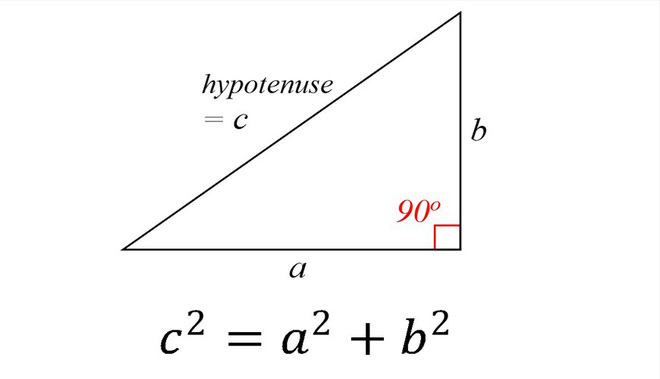
\includegraphics[scale=0.5]{images/pytago}
        \end{center}
        \caption{Hình minh họa} \label{Fig:Hinh-minh-hoa}
      \end{figure}

      Hình ảnh minh họa (Hình \ref{Fig:Hinh-minh-hoa}).
    \end{itemize}

  \section{Tham chiếu bảng}
    \begin{itemize}
      \item Sử dụng các môi trường \verb|table| để viết công chèn bảng, rồi đặt lệnh \verb|\label{Tab:Name Label}| vào trong mỗi môi trường. Để tham chiếu lại bảng thì dùng lệnh \verb|\ref{Tab:Name Label}|.
      \item Code mẫu:
        \begin{verbatim}
          \begin{table}[htp]
            \begin{center}
              % Chèn bảng vào đây
            \end{center}
            \caption{Bảng minh họa} \label{Tab:Bang-minh-hoa}
          \end{table}
    
          Bảng minh họa (Bảng \ref{Tab:Bang-minh-hoa}).
        \end{verbatim}
      \item Kết quả cho đoạn code ở trên:
        
      \begin{table}[!htp]
        \caption{Bảng minh họa} \label{Tab:Bang-minh-hoa}
        \begin{center}
          {
            \renewcommand{\arraystretch}{1.3}
            \begin{tabular}{|c|c|c|c|c|} \hline
              \(a\) & \(b\) & \(c\) & \(a^2 + b^2\) & \(c^2\) \\ \hline
              3 & 4 & 5 & \(3^2 + 4^2 = 25\) & \(5^2 = 25\) \\ \hline
            \end{tabular}
          }
        \end{center}
      \end{table}

      Bảng minh họa (Bảng \ref{Tab:Bang-minh-hoa}).
    \end{itemize}
\end{document}